\item \underline{Correas de Techo. Caso con Tillas en el centro de la luz}\\
\begin{itemize}
\item El primer estado de carga corresponde a peso propio + sobrecarga.

\begin{figure}[H]
\begin{center}
     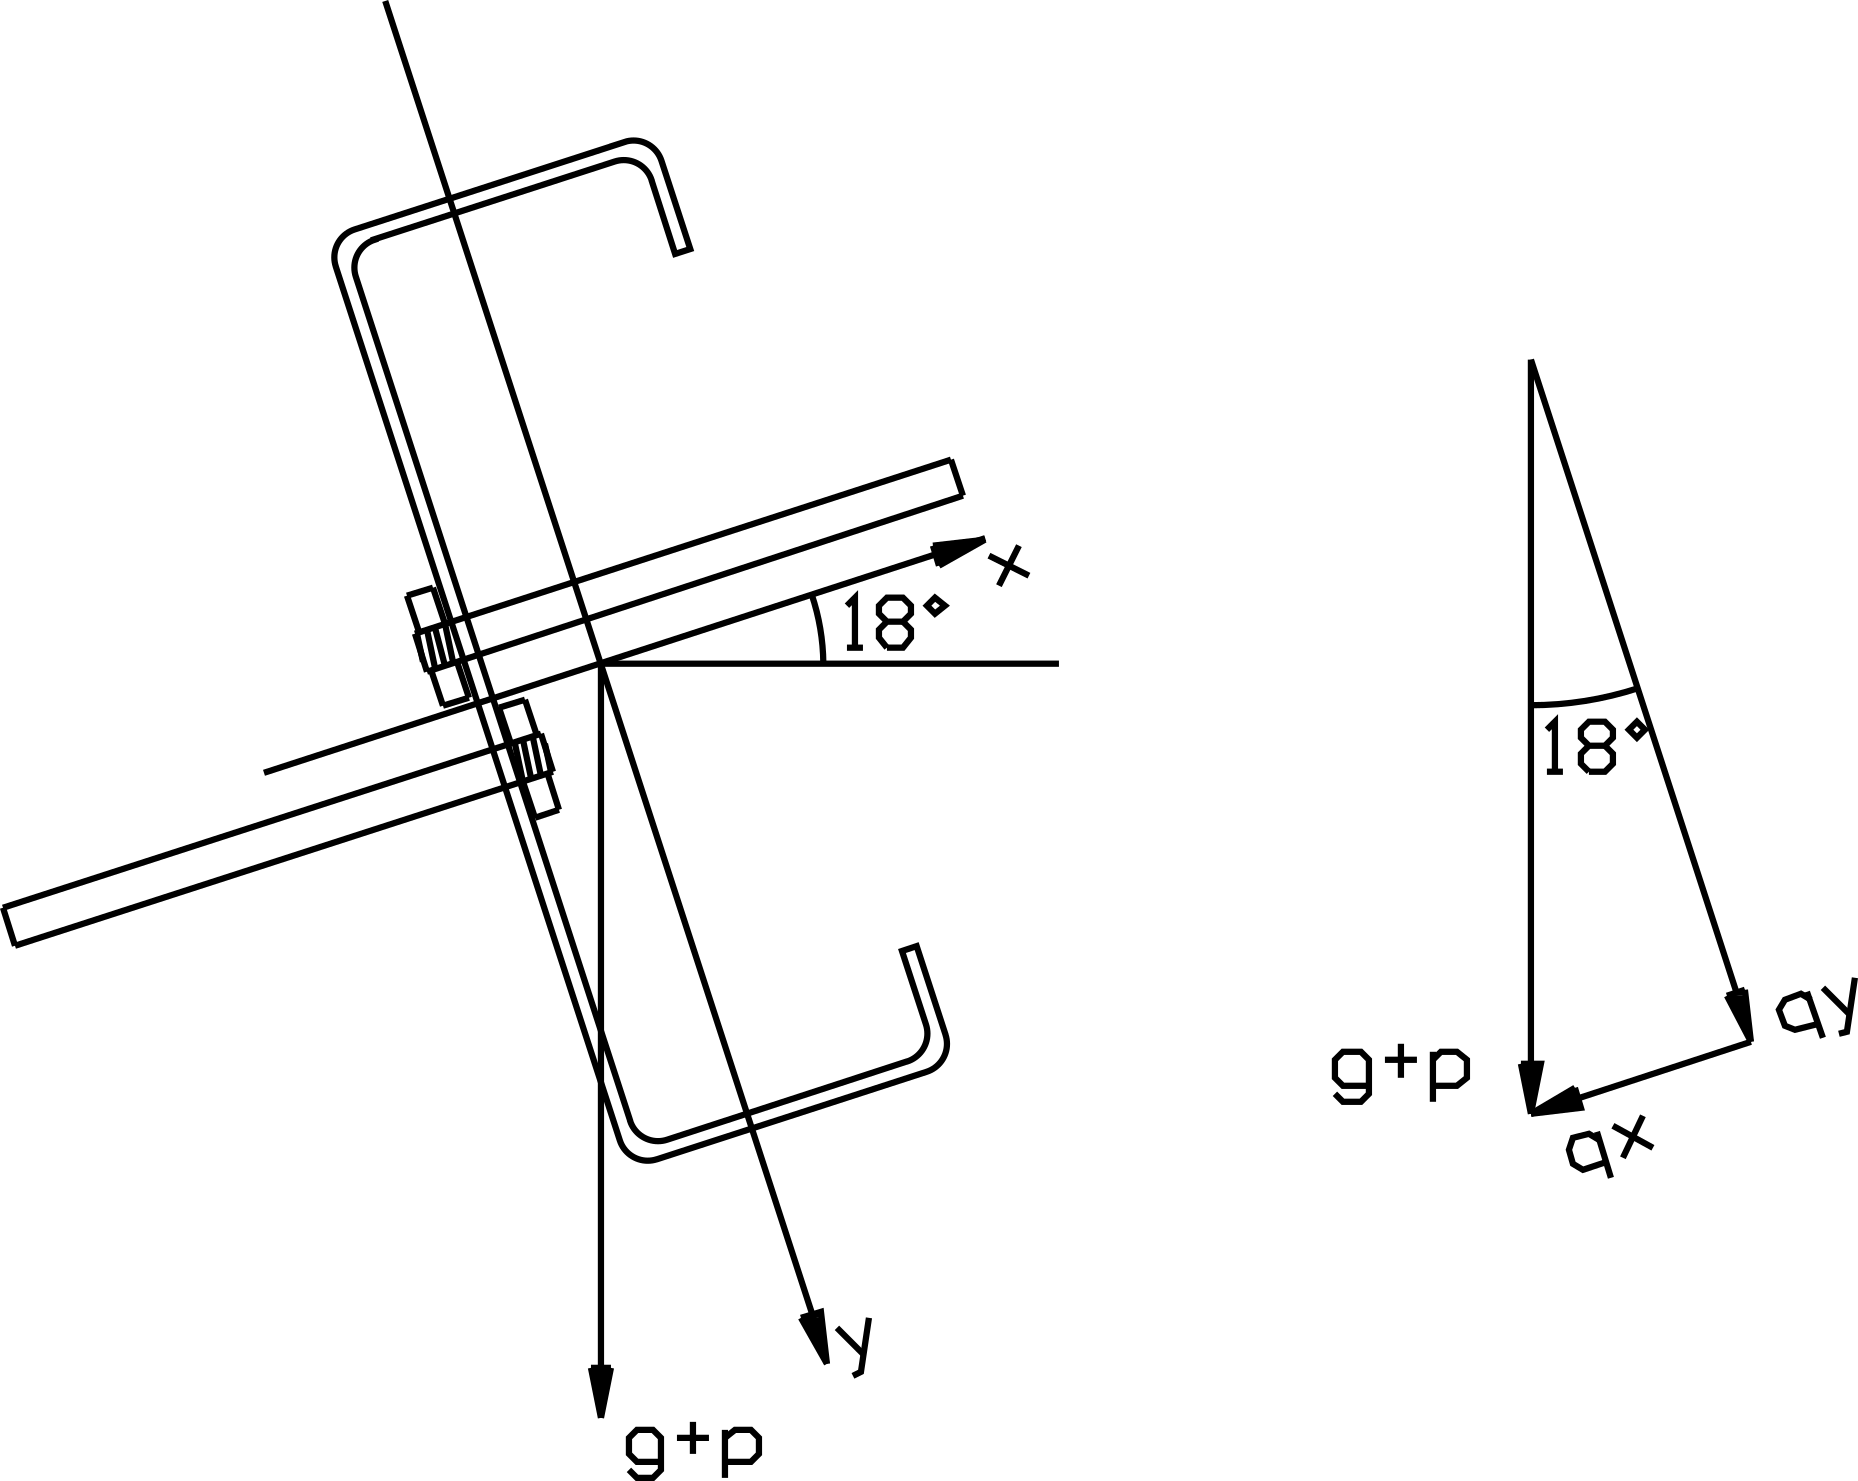
\includegraphics[scale = 1]{chapters/chapter_2/images/figura3.png}
\caption{Correa de techo con tillas - Estado: peso propio + sobrecarga}
\end{center}
\end{figure}

$$q= (g+p)\cdot s = (14 \frac{Kg}{m^2}+30 \frac{Kg}{m^2}) \cdot 1.05m = \framebox{$46.2 \frac{Kg}{m}$}$$
Descomponiendo la resultante en las direcciones $x$ e $y$ tenemos:
\begin{align*}
& q_x=q \cdot Sen \alpha= 46.2 \frac{Kg}{m} \cdot Sen(18\textsuperscript{o})= \framebox{$14.27 \frac{Kg}{m}$}\\
& q_y=q \cdot Cos \alpha= 46.2 \frac{Kg}{m} \cdot Cos(18\textsuperscript{o})= \framebox{$43.93 \frac{Kg}{m}$}
\end{align*}

Procedemos a calcular los momentos en el centro de la luz, producidos por cada una de estas cargas lineales, suponemos que las correas se encuentran simplemente apoyadas.
\begin{align*}
& M_x= \frac{q_y \cdot l^2}{8} = \frac{43.93 \frac{Kg}{m} \cdot (5m)^2}{8} = \framebox{$137.28 Kg.m$} \\
& M_y= \frac{q_x \cdot l^2}{8} = \frac{14.27 \frac{Kg}{m} \cdot (\frac{5m}{2})^2}{8} = \framebox{$11.14 Kg.m$}
\end{align*}

\newpage
\item El segundo estado de carga corresponde a peso propio + viento.

\begin{figure}[H]
\begin{center}
     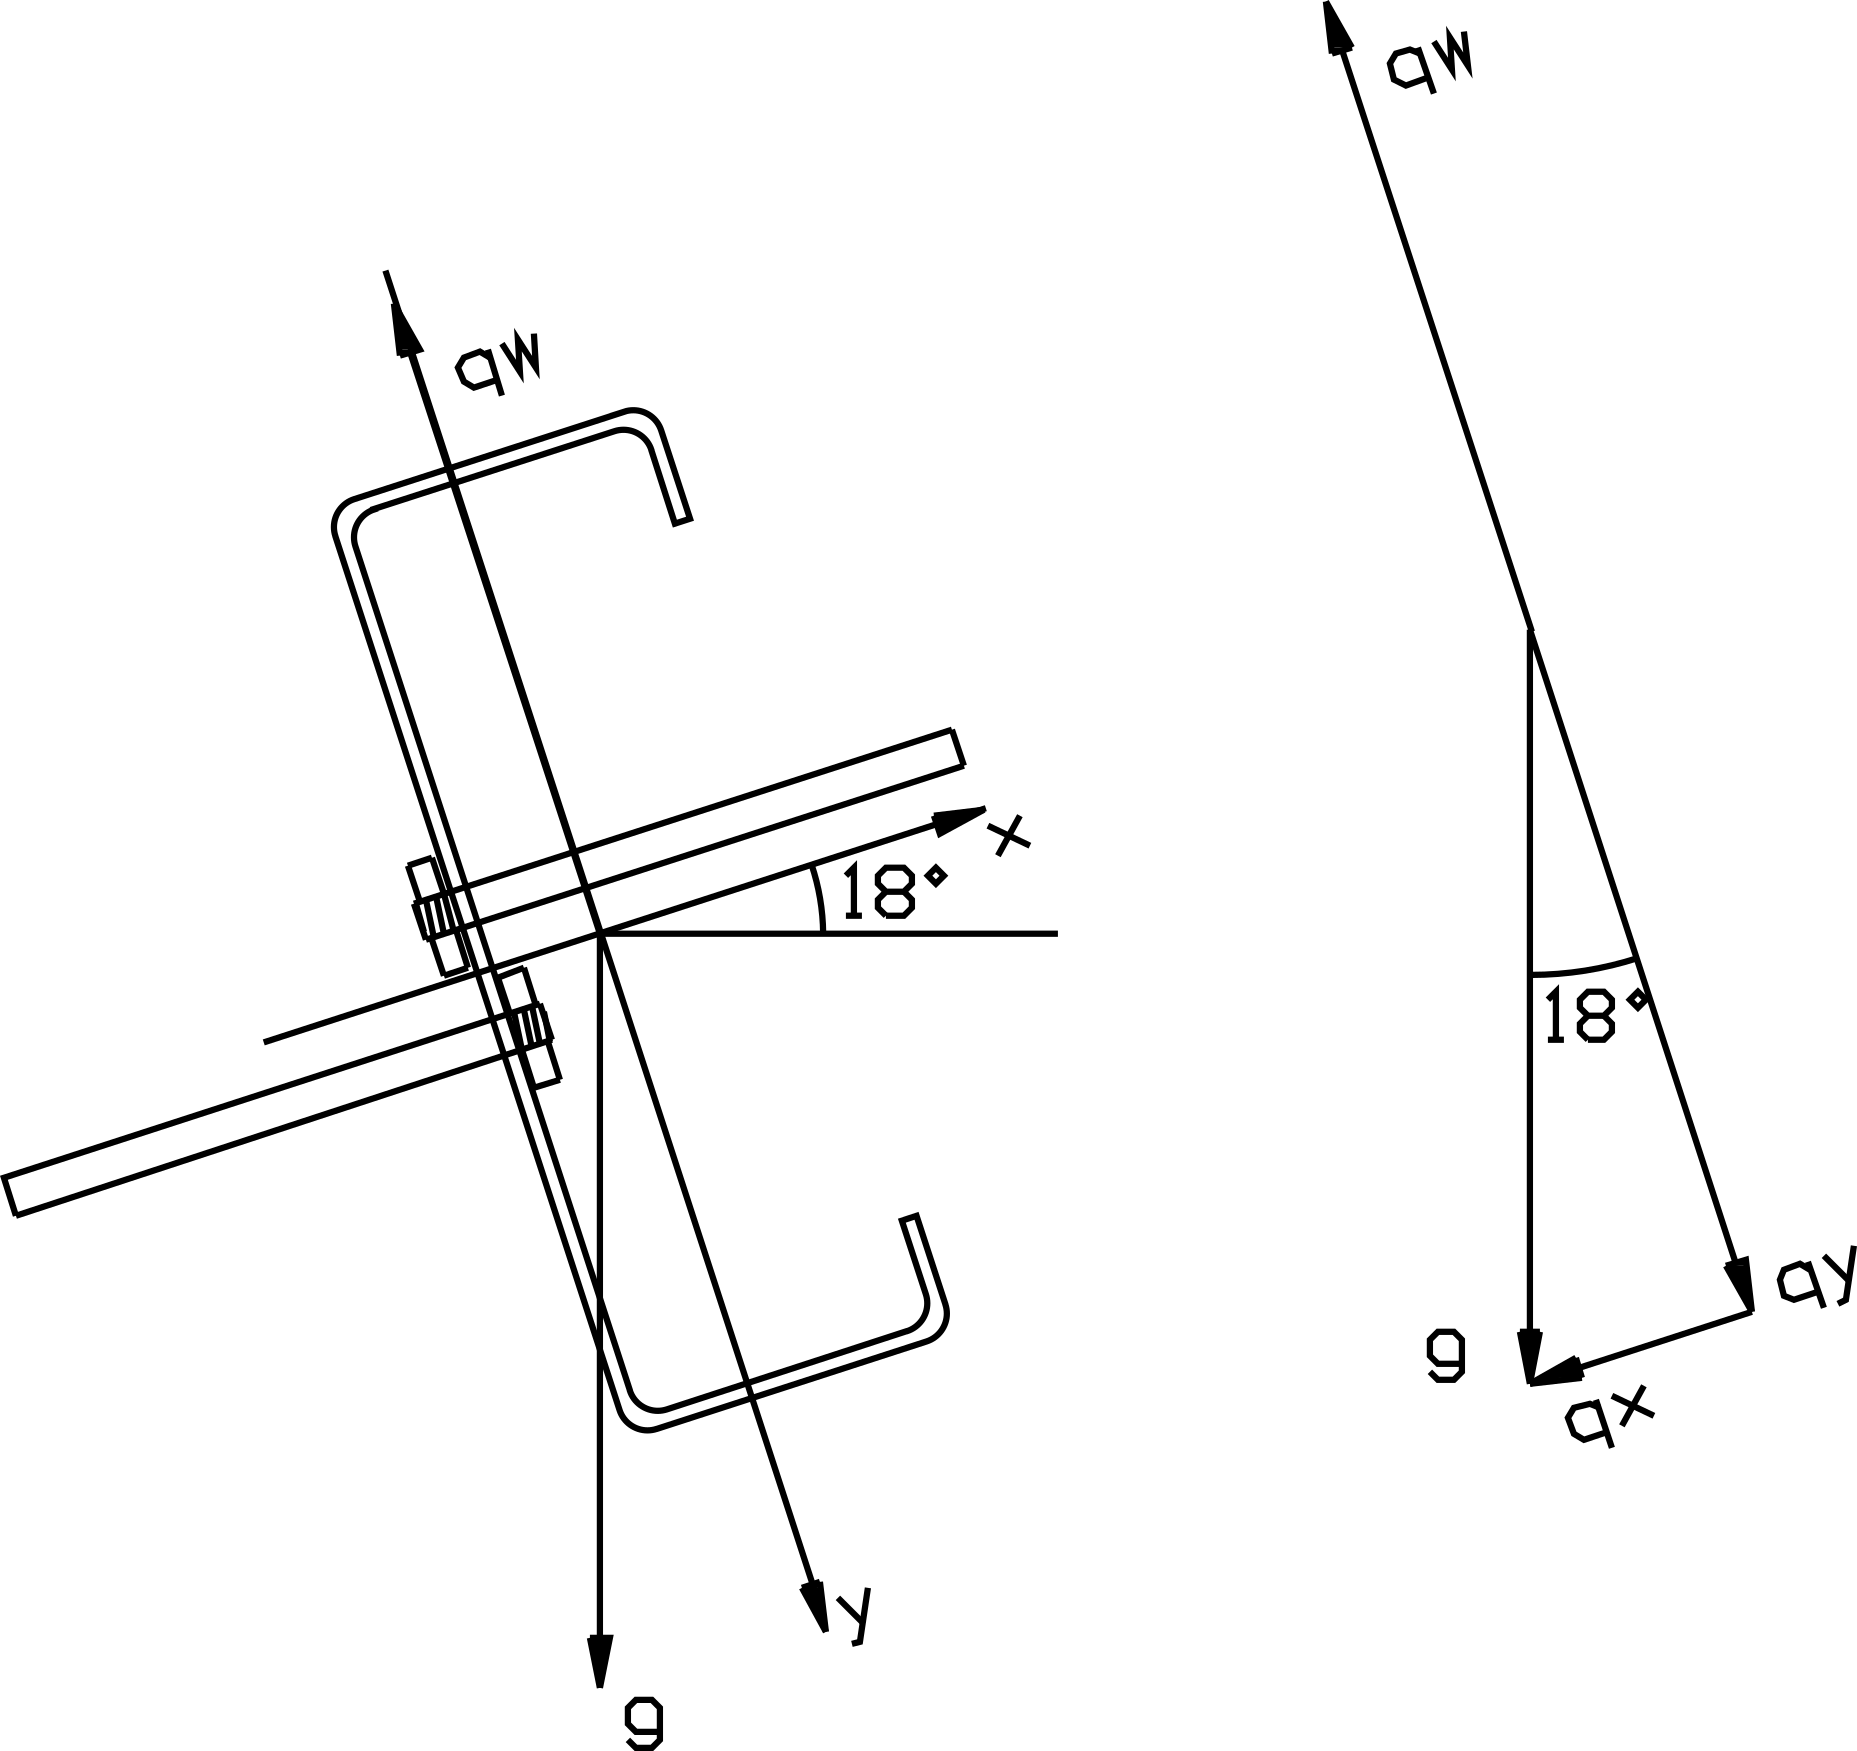
\includegraphics[scale = 1]{chapters/chapter_2/images/figura4.png}
\caption{Correa de techo con tillas - Estado: peso propio + viento}
\end{center}
\end{figure}

Descomponiendo la resultante en las direcciones $x$ e $y$ tenemos:
\begin{align*}
& q_x=g \cdot Sen \alpha \cdot s = 14 \frac{Kg}{m^2} \cdot Sen(18\textsuperscript{o}) \cdot 1.05m= \framebox{$4.54 \frac{Kg}{m}$}\\
& q_y=(q_w - g \cdot Cos \alpha) \cdot s = (175 \frac{Kg}{m^2} - 14 \frac{Kg}{m^2} \cdot Cos(18\textsuperscript{o}) \cdot 1.05m= \framebox{$169.76 \frac{Kg}{m}$}
\end{align*}

Procedemos a calcular los momentos en el centro de la luz, producidos por cada una de estas cargas lineales, suponemos que las correas se encuentran simplemente apoyadas.

\begin{align*}
& M_x= \frac{q_y \cdot l^2}{8} = \frac{169.76 \frac{Kg}{m} \cdot (5m)^2}{8} = \framebox{$530.5 Kg.m$} \\
& M_y= \frac{q_x \cdot l^2}{8} = \frac{4.54 \frac{Kg}{m} \cdot (\frac{5m}{2})^2}{8} = \framebox{$3.54 Kg.m$}
\end{align*}

\item Tension admisible.\\
Dado que se utiliza acero F-24, tenemos según el reglamento CIRSOC 301 una tensión de fluencia $\sigma_{fl}=2400 \frac{Kg}{cm^2}$ y tomando un coeficiente de seguridad $\gamma = 1.6$ , se obtiene una tensión admisible de:
$$\sigma_{adm}= \frac{\sigma_{fl}}{\gamma} = \frac{2400 \frac{Kg}{cm^2}}{1.6} = \framebox{$1500 \frac{Kg}{cm^2}$}$$

\newpage
\item Selección de la correa.\\
Adoptamos un perfil \framebox{C 180-70-25-2.5} de chapa doblada, con las siguientes características:
\begin{align*}
& W_x= 48.912 cm^3 \\
& W_y= 12.945 cm^3 \\
& J_x= 440.204 cm^4 \\
& J_y= 61.373 cm^4
\end{align*}

\item Verificamos las tensiones para ambos estados de carga.\\
\underline{Estado de carga 1: peso propio + sobrecarga}
\begin{align*}
& \sigma_x=\frac{M_x}{W_x} = \frac{13728 Kg.cm}{48.912 cm^3} = 280.66 \frac{Kg}{cm^2}\\
& \sigma_y=\frac{M_y}{W_y} = \frac{1114 Kg.cm}{12.945 cm^3} = 86.05 \frac{Kg}{cm^2}\\
& \sigma_t= \sigma_x + \sigma_y = 280.66 \frac{Kg}{cm^2} + 86.05 \frac{Kg}{cm^2} = \framebox{$366.72 \frac{Kg}{cm^2}$}\\
& \sigma_t < \sigma_{adm}\\
& 366.72 \frac{Kg}{cm^2} < 1500 \frac{Kg}{cm^2} \Rightarrow \text{Verifica} \quad \surd
\end{align*}

\underline{Estado de carga 2: peso propio + viento}
\begin{align*}
& \sigma_x=\frac{M_x}{W_x} = \frac{53050 Kg.cm}{48.912 cm^3} = 1084.60 \frac{Kg}{cm^2}\\
& \sigma_y=\frac{M_y}{W_y} = \frac{354 Kg.cm}{12.945 cm^3} = 27.34 \frac{Kg}{cm^2}\\
& \sigma_t= \sigma_x + \sigma_y = 1084.60 \frac{Kg}{cm^2} + 27.34 \frac{Kg}{cm^2} = \framebox{$1111.94 \frac{Kg}{cm^2}$}\\
& \sigma_t < \sigma_{adm}\\
& 1111.94 \frac{Kg}{cm^2} < 1500 \frac{Kg}{cm^2} \Rightarrow \text{Verifica} \quad \surd
\end{align*}

\item Verificamos las deformaciones para ambos estados de carga.\\
La flecha admisible de cumplir $f < \frac{l}{300} \Rightarrow f < \frac{5m}{300} \Rightarrow f < 1.66cm$\\
Para el cálculo de la flecha utilizaremos la expresión $f= \frac{5}{384} \cdot \frac{q \cdot l^4}{E \cdot J}$\\

\underline{Estado de carga 1: peso propio + sobrecarga}
\begin{align*}
& f_x=0 \\
& f_y=\frac{5}{384} \cdot \frac{q_y \cdot l^4}{E \cdot J_x}\\
& f_y=\frac{5}{384} \cdot \frac{0.4393 \frac{Kg}{cm} \cdot (500cm)^4}{2100000 \frac{Kg}{cm^2} \cdot 440.204 cm^4} = 0.38cm\\
& f = \sqrt{f_x^2+f_y^2} = \framebox{$0.38cm$}\\
& f < f_{adm}\\
& 0.38cm < 1.66cm \Rightarrow \text{Verifica} \quad \surd
\end{align*}

\underline{Estado de carga 2: peso propio + viento}
\begin{align*}
& f_x= 0 \\
& f_y=\frac{5}{384} \cdot \frac{q_y \cdot l^4}{E \cdot J_x}\\
& f_y=\frac{5}{384} \cdot \frac{1.6976 \frac{Kg}{cm} \cdot (500cm)^4}{2100000 \frac{Kg}{cm^2} \cdot 440.204 cm^4} = 1.49cm\\
& f = \sqrt{f_x^2+f_y^2} = \framebox{$1.49cm$}\\
& f < f_{adm}\\
& 1.49cm < 1.66cm \Rightarrow \text{Verifica} \quad \surd
\end{align*}
Por lo tanto verifica el requerimiento de deformación especificado en el reglamento.\\
\end{itemize}
